\documentclass[letterpaper]{article}
\usepackage{graphicx}
\usepackage{tikz}
\usepackage[margin=2cm]{geometry}
\usepackage{xcolor}
%\usepackage{tgpagella} % No se usa actualmente
\usepackage{fourier}
%\usepackage{charter}   % No se usa actualmente
\usepackage{tgheros}
\usepackage[T1]{fontenc}
\usepackage[utf8]{inputenc}
\usepackage{setspace}
\usepackage[spanish, es-tabla]{babel} % es-tabla pone "Tabla" en vez de "Cuadro"
\usepackage{multicol}
\usepackage{booktabs}
\usepackage{caption}
\usepackage{tocloft}
\usepackage{placeins}
\usepackage{float}
\usepackage[hidelinks]{hyperref} % 'hidelinks' quita los cuadros de colores feos

% Puntos guía entre el texto de la entrada y el número de página.
\renewcommand{\cftsecleader}{\cftdotfill{\cftdotsep}}
\renewcommand{\cftfigleader}{\cftdotfill{\cftdotsep}}
\renewcommand{\cfttableader}{\cftdotfill{\cftdotsep}}
\setlength{\cftsecindent}{2em}  % Sangría para secciones en el índice
\setlength{\textfloatsep}{8pt}   % espacio entre float arriba/abajo y texto
\setlength{\intextsep}{8pt}      % espacio para figuras "en medio" del texto ([h])
\usepackage{fancyhdr}

\pagestyle{fancy}
\fancyhead{} % Borra el encabezado por defecto
\fancyhead[L]{\textbf{Estadística II 2026-2}} % Encabezado izquierdo
\fancyhead[R]{Actividad 3: Análisis de regresión lineal}
\definecolor{azulunam}{RGB}{0, 43, 122}
\definecolor{doradounam}{RGB}{199, 146, 19}


\begin{document}

    \begin{titlepage}
        \thispagestyle{empty}
        \fontfamily{qhv}\selectfont
        \singlespacing
        \fontsize{14}{18}\selectfont
        %\newgeometry{margin=2cm} % márgenes más pequeños
        \newgeometry{
            left=1cm,
            right=1cm,
            top=1cm,
            bottom=1cm
        }

        \begin{tikzpicture}[remember picture, overlay]
            \node[anchor=center] 
            at ([xshift=8.2cm,yshift=11.5cm]current page.center) {
                
\includegraphics[height=2cm]{escudo_mac.jpg}
            };
            \node[anchor=center] 
            at ([xshift=-8.6cm,yshift=11.5cm]current page.center) {
                
\includegraphics[height=2.6cm]{escudo-a.png}
            };
            % Linea horizontal
            \draw[line width=2pt, color=azulunam] 
            ([xshift=-6.5cm,yshift=11.5cm]current page.center) -- 
            ([xshift=6.2cm,yshift=11.5cm]current page.center);
            %Linea vertical
            \draw[line width=2pt, color=azulunam] 
            ([xshift=-8.6cm,yshift=-11cm]current page.center) -- 
            ([xshift=-8.6cm,yshift=9.5cm]current page.center);
        \end{tikzpicture}
        \begin{center}
            {\Large \textbf{\textsc{UNIVERSIDAD NACIONAL AUTÓNOMA DE MÉXICO}} \vspace{0.8cm} }\\
            {\large \textbf{\textsc{FACULTAD DE ESTUDIOS SUPERIORES ACATLÁN}} \vspace{0.8cm} }\\
            \vspace{1cm}
            {\textsc{División de Matemáticas e Ingenierias}} \\
            \vspace{0.8cm}
            Licenciatura en Matemáticas Aplicadas y Computación \\
            \vspace{0.8cm}

            \begin{minipage}{0.8\textwidth}
                \centering
                Asignatura: Estadística II \\
                \vspace{0.3cm}
                Profesor: Jaime Vergara Prado
            \end{minipage}\\
            \vspace{0.8cm}
            {\huge Actividad 3: \\ \vspace{0.3cm} Análisis de regresión lineal}

            \begin{table}[h]
                \centering
                \vspace{0.3cm}
                {\fontsize{15}{18}\selectfont
                \begin{tabular}{l c c} % 'l' izquierda, 'c' centro, 'c' centro
                    % No ponemos '|' entre las letras para evitar líneas verticales
                    
                    Presenta: &  Cortés Cortés Bryan Yael\\
                    %\addlinespace[0.3cm] % Espacio extra entre filas sin líneas
                       &  Pineda Ortega Daniel\\
                       &  Rodríguez Mérida Diego\\
                       &  Romero Minchaca Esteban\\
                       &  Sánchez Santos Denisse Alejandra\\
                       &  Suriano Granados Duncan Zuriel
                    
                \end{tabular}
                }
            \end{table}

            \begin{table}[h]
                \centering
                \caption*{Registro de evaluación}
                \renewcommand{\arraystretch}{1.5} % 1 es el normal, 1.5 es ideal
                \begin{tabular}{|l|c|c|r|} % Las barras '|' crean las líneas verticales
                    \hline % Línea horizontal superior
                    Nombre & Evaluación & Inasistencia & Evaluación total\\ \hline \hline
                    Cortés Cortés Bryan Yael          & 100 \%                 & 0\%            & 0\%\\ \hline
                    Pineda Ortega Daniel          & 100 \%                 & 0\%            & 0\%\\ \hline
                    Rodríguez Mérida Diego          & 100 \%                 & 0\%            & 0\%\\ \hline
                    Romero Minchaca Esteban          & 100 \%                 & 0\%            & 0\%\\ \hline
                    Sánchez Santos Denisse Alejandra          & 100 \%                 & 0\%            & 0\%\\ \hline
                    Suriano Granados Duncan Zuriel          & 100 \%                 & 0\%            & 0\%\\ \hline
                \end{tabular}
            \end{table} \vspace{0.8cm}

            Grupo: 2651 \\ \vspace{0.8cm}
            \hspace{5cm} Fecha de entrega: 09 de abril de 2026 

            
        \end{center}
            
    
        \restoregeometry
    \end{titlepage}

    \pagenumbering{roman} % Números romanos para el índice (opcional)
    \tableofcontents
   
    \listoffigures %(Índice de imágenes).

    \listoftables %(Índice de tablas).

     \newpage

    \pagenumbering{arabic} % Volver a números normales (1, 2, 3...)
    \section*{Introducción}
    \phantomsection
    \addcontentsline{toc}{section}{Introducción}
    % Al dar click en "Introducción" en el índice, el PDF te llevará aquí.
    Lorem ipsum dolor sit amet, consectetur adipiscing elit. Sed do eiusmod tempor incididunt ut labore et dolore 
    magna aliqua. Ut enim ad minim veniam, quis nostrud exercitation ullamco laboris nisi ut aliquip ex ea commodo 
    consequat. Duis aute irure dolor in reprehenderit in voluptate velit esse cillum dolore eu fugiat nulla pariatur. 
    Excepteur sint occaecat cupidatat non proident, sunt in culpa qui officia deserunt mollit anim id est laborum.\\ \\
    \textbf{¿Qué es Lorem Ipsum?}
    Lorem Ipsum es simplemente el texto de relleno de las imprentas y archivos de texto. Lorem Ipsum ha sido el texto 
    de relleno estándar de las industrias desde el año 1500, cuando un impresor (N. del T. persona que se dedica a la imprenta) 
    desconocido usó una galería de textos y los mezcló de tal manera que logró hacer un libro de textos especimen. 
    No sólo sobrevivió 500 años, sino que tambien ingresó como texto de relleno en documentos electrónicos, quedando 
    esencialmente igual al original. Fue popularizado en los 60s con la creación de las hojas "Letraset", las cuales 
    contenian pasajes de Lorem Ipsum, y más recientemente con software de autoedición, como por ejemplo Aldus PageMaker, 
    el cual incluye versiones de Lorem Ipsum.\\ \\

    \textbf{¿Por qué lo usamos?}
    Es un hecho establecido hace demasiado tiempo que un lector se distraerá con el contenido del texto de un sitio 
    mientras que mira su diseño. El punto de usar Lorem Ipsum es que tiene una distribución más o menos normal de las 
    letras, al contrario de usar textos como por ejemplo "Contenido aquí, contenido aquí". Estos textos hacen parecerlo 
    un español que se puede leer. Muchos paquetes de autoedición y editores de páginas web usan el Lorem Ipsum como 
    su texto por defecto, y al hacer una búsqueda de "Lorem Ipsum" va a dar por resultado muchos sitios web que usan 
    este texto si se encuentran en estado de desarrollo. Muchas versiones han evolucionado a través de los años, algunas 
    veces por accidente, otras veces a propósito (por ejemplo insertándole humor y cosas por el estilo). \\ \\


    \textbf{¿De dónde viene?}
    Al contrario del pensamiento popular, el texto de Lorem Ipsum no es simplemente texto aleatorio. Tiene sus raices en 
    una pieza cl´sica de la literatura del Latin, que data del año 45 antes de Cristo, haciendo que este adquiera mas de 
    2000 años de antiguedad. Richard McClintock, un profesor de Latin de la Universidad de Hampden-Sydney en Virginia, 
    encontró una de las palabras más oscuras de la lengua del latín, "consecteur", en un pasaje de Lorem Ipsum, y al seguir 
    leyendo distintos textos del latín, descubrió la fuente indudable. Lorem Ipsum viene de las secciones 1.10.32 y 1.10.33 
    de "de Finnibus Bonorum et Malorum" (Los Extremos del Bien y El Mal) por Cicero, escrito en el año 45 antes de Cristo. 
    Este libro es un tratado de teoría de éticas, muy popular durante el Renacimiento. La primera linea del Lorem Ipsum, 
    "Lorem ipsum dolor sit amet..", viene de una linea en la sección 1.10.32 \\ \\ 

    El trozo de texto estándar de Lorem Ipsum usado desde el año 1500 es reproducido debajo para aquellos interesados. 
    Las secciones 1.10.32 y 1.10.33 de "de Finibus Bonorum et Malorum" por Cicero son también reproducidas en su forma original 
    exacta, acompañadas por versiones en Inglés de la traducción realizada en 1914 por H. Rackham. \\ \\

    \textbf{¿Dónde puedo conseguirlo?}
    Hay muchas variaciones de los pasajes de Lorem Ipsum disponibles, pero la mayoría sufrió alteraciones en alguna manera, 
    ya sea porque se le agregó humor, o palabras aleatorias que no parecen ni un poco creíbles. Si vas a utilizar un pasaje 
    de Lorem Ipsum, necesitás estar seguro de que no hay nada avergonzante escondido en el medio del texto. Todos los generadores 
    de Lorem Ipsum que se encuentran en Internet tienden a repetir trozos predefinidos cuando sea necesario, haciendo a este 
    el único generador verdadero (válido) en la Internet. Usa un diccionario de mas de 200 palabras provenientes del latín, 
    combinadas con estructuras muy útiles de sentencias, para generar texto de Lorem Ipsum que parezca razonable. 
    Este Lorem Ipsum generado siempre estará libre de repeticiones, humor agregado o palabras no características del lenguaje, etc.
    5 párrafos palabras bytes listas Comenzar con 'Lorem ipsum dolor sit amet...'

    \section{Desarrollo}
    Lorem ipsum dolor sit amet, consectetur adipiscing elit. Vestibulum ipsum quam, finibus sed purus in, viverra eleifend sem. 
    Nulla feugiat lacinia nulla, sed tempus erat tempor id. Phasellus eget consectetur urna. Etiam eu rutrum nulla. In malesuada 
    diam id augue maximus, quis convallis metus fringilla. Vivamus vitae congue dolor. Sed et sagittis metus, ac mollis quam. 
    Donec vestibulum neque diam, lobortis vestibulum nunc vehicula eu. Proin ornare mauris ac nibh dapibus, id tincidunt erat 
    eleifend. Maecenas egestas nunc nibh, ac dictum neque gravida vitae. Praesent posuere ligula ut faucibus pretium. Mauris lorem 
    ante, vulputate in orci at, gravida aliquet odio. Duis eget dolor non tellus euismod varius sed id magna. Interdum et malesuada 
    fames ac ante ipsum primis in faucibus. Integer eu massa eleifend, imperdiet mauris vel, dictum neque.
    Donec quis sodales augue. Sed euismod vehicula ultricies. Aenean hendrerit sem lectus, sed commodo justo elementum id. 
    In ultricies ipsum malesuada velit ornare euismod. Fusce eget finibus quam, sed aliquet ligula. Nullam accumsan tellus accumsan 
    magna mollis eleifend. Cras semper nulla dignissim metus consectetur semper. Fusce vel tortor sem. Mauris pharetra cursus orci 
    vel rhoncus. Suspendisse vel massa et velit ultrices consequat in et elit. Proin eu ex ut est porta efficitur. Duis ut malesuada 
    purus. Pellentesque sed magna eget felis suscipit eleifend a at libero. Maecenas ut interdum est. Integer pharetra, leo et 
    tristique posuere, lacus urna sagittis nisl, et vehicula dolor ipsum sit amet nunc. Nam vitae aliquam erat, id blandit nisl.

    Sed in varius tellus. Nullam vehicula lorem a augue bibendum, non blandit magna faucibus. Donec vitae blandit orci, nec tempor 
    felis. Nulla vitae ultrices erat, sit amet sollicitudin purus. Maecenas bibendum in magna id aliquet. Donec cursus lacus congue 
    ligula efficitur porta. Sed enim orci, porttitor sed ex id, bibendum dignissim elit. Curabitur pretium nulla vel nisi ornare 
    imperdiet quis vitae lacus. Proin a nisl euismod, venenatis eros id, malesuada ex. Curabitur suscipit pellentesque pretium. 
    Pellentesque bibendum est vel nisl porta luctus. Vestibulum varius tincidunt nulla vitae ornare. Vestibulum ante ipsum primis 
    in faucibus orci luctus et ultrices posuere cubilia curae; Sed volutpat id eros ac vestibulum. Quisque auctor nulla interdum 
    tempor blandit.

    Cras dictum varius purus, scelerisque sodales tortor elementum commodo. Ut dui sem, sagittis sed diam nec, scelerisque suscipit 
    metus. Interdum et malesuada fames ac ante ipsum primis in faucibus. Nullam sollicitudin felis vel dui rutrum elementum. Proin 
    turpis sapien, blandit at mi ac, pellentesque scelerisque nibh. Nulla maximus suscipit luctus. Integer in velit laoreet, posuere 
    odio vitae, iaculis mauris. Duis in erat vulputate, pretium elit sed, maximus risus. Aenean eu commodo sem, nec iaculis sem. 
    Nullam sagittis, tortor fermentum rhoncus mollis, nulla arcu lobortis felis, nec molestie dui tortor at dolor. Donec lorem neque, 
    facilisis nec facilisis vitae, faucibus condimentum quam. Vestibulum sodales sapien nec ex eleifend, et dapibus orci efficitur. 
    Morbi pellentesque lectus in nisl fermentum, at commodo odio vehicula. Duis rhoncus malesuada diam, non efficitur metus porttitor 
    vitae. Suspendisse venenatis nibh vitae purus tincidunt condimentum. Curabitur iaculis nunc id convallis cursus.

    Aliquam erat volutpat. In hac habitasse platea dictumst. Vivamus semper magna sit amet enim dignissim, in faucibus velit sodales. 
    Praesent a erat quam. Ut lorem quam, ultrices ut lorem sit amet, sodales posuere metus. Vivamus non congue dolor. Fusce facilisis 
    sed lectus at commodo. Nam mauris nunc, fringilla aliquet rutrum at, sodales vel lacus. Ut ultricies sollicitudin dolor, a mollis 
    odio gravida tempor. Sed non lacus quam. Aenean ante justo, auctor vitae nunc eget, posuere molestie ante. Sed finibus, magna a 
    rhoncus imperdiet, erat massa ullamcorper risus, vitae pretium augue enim vel enim.
    % Una sola imagen centrada con su respectiva leyenda y etiqueta para referenciarla en el texto.
    \begin{figure}[h]
    \centering
    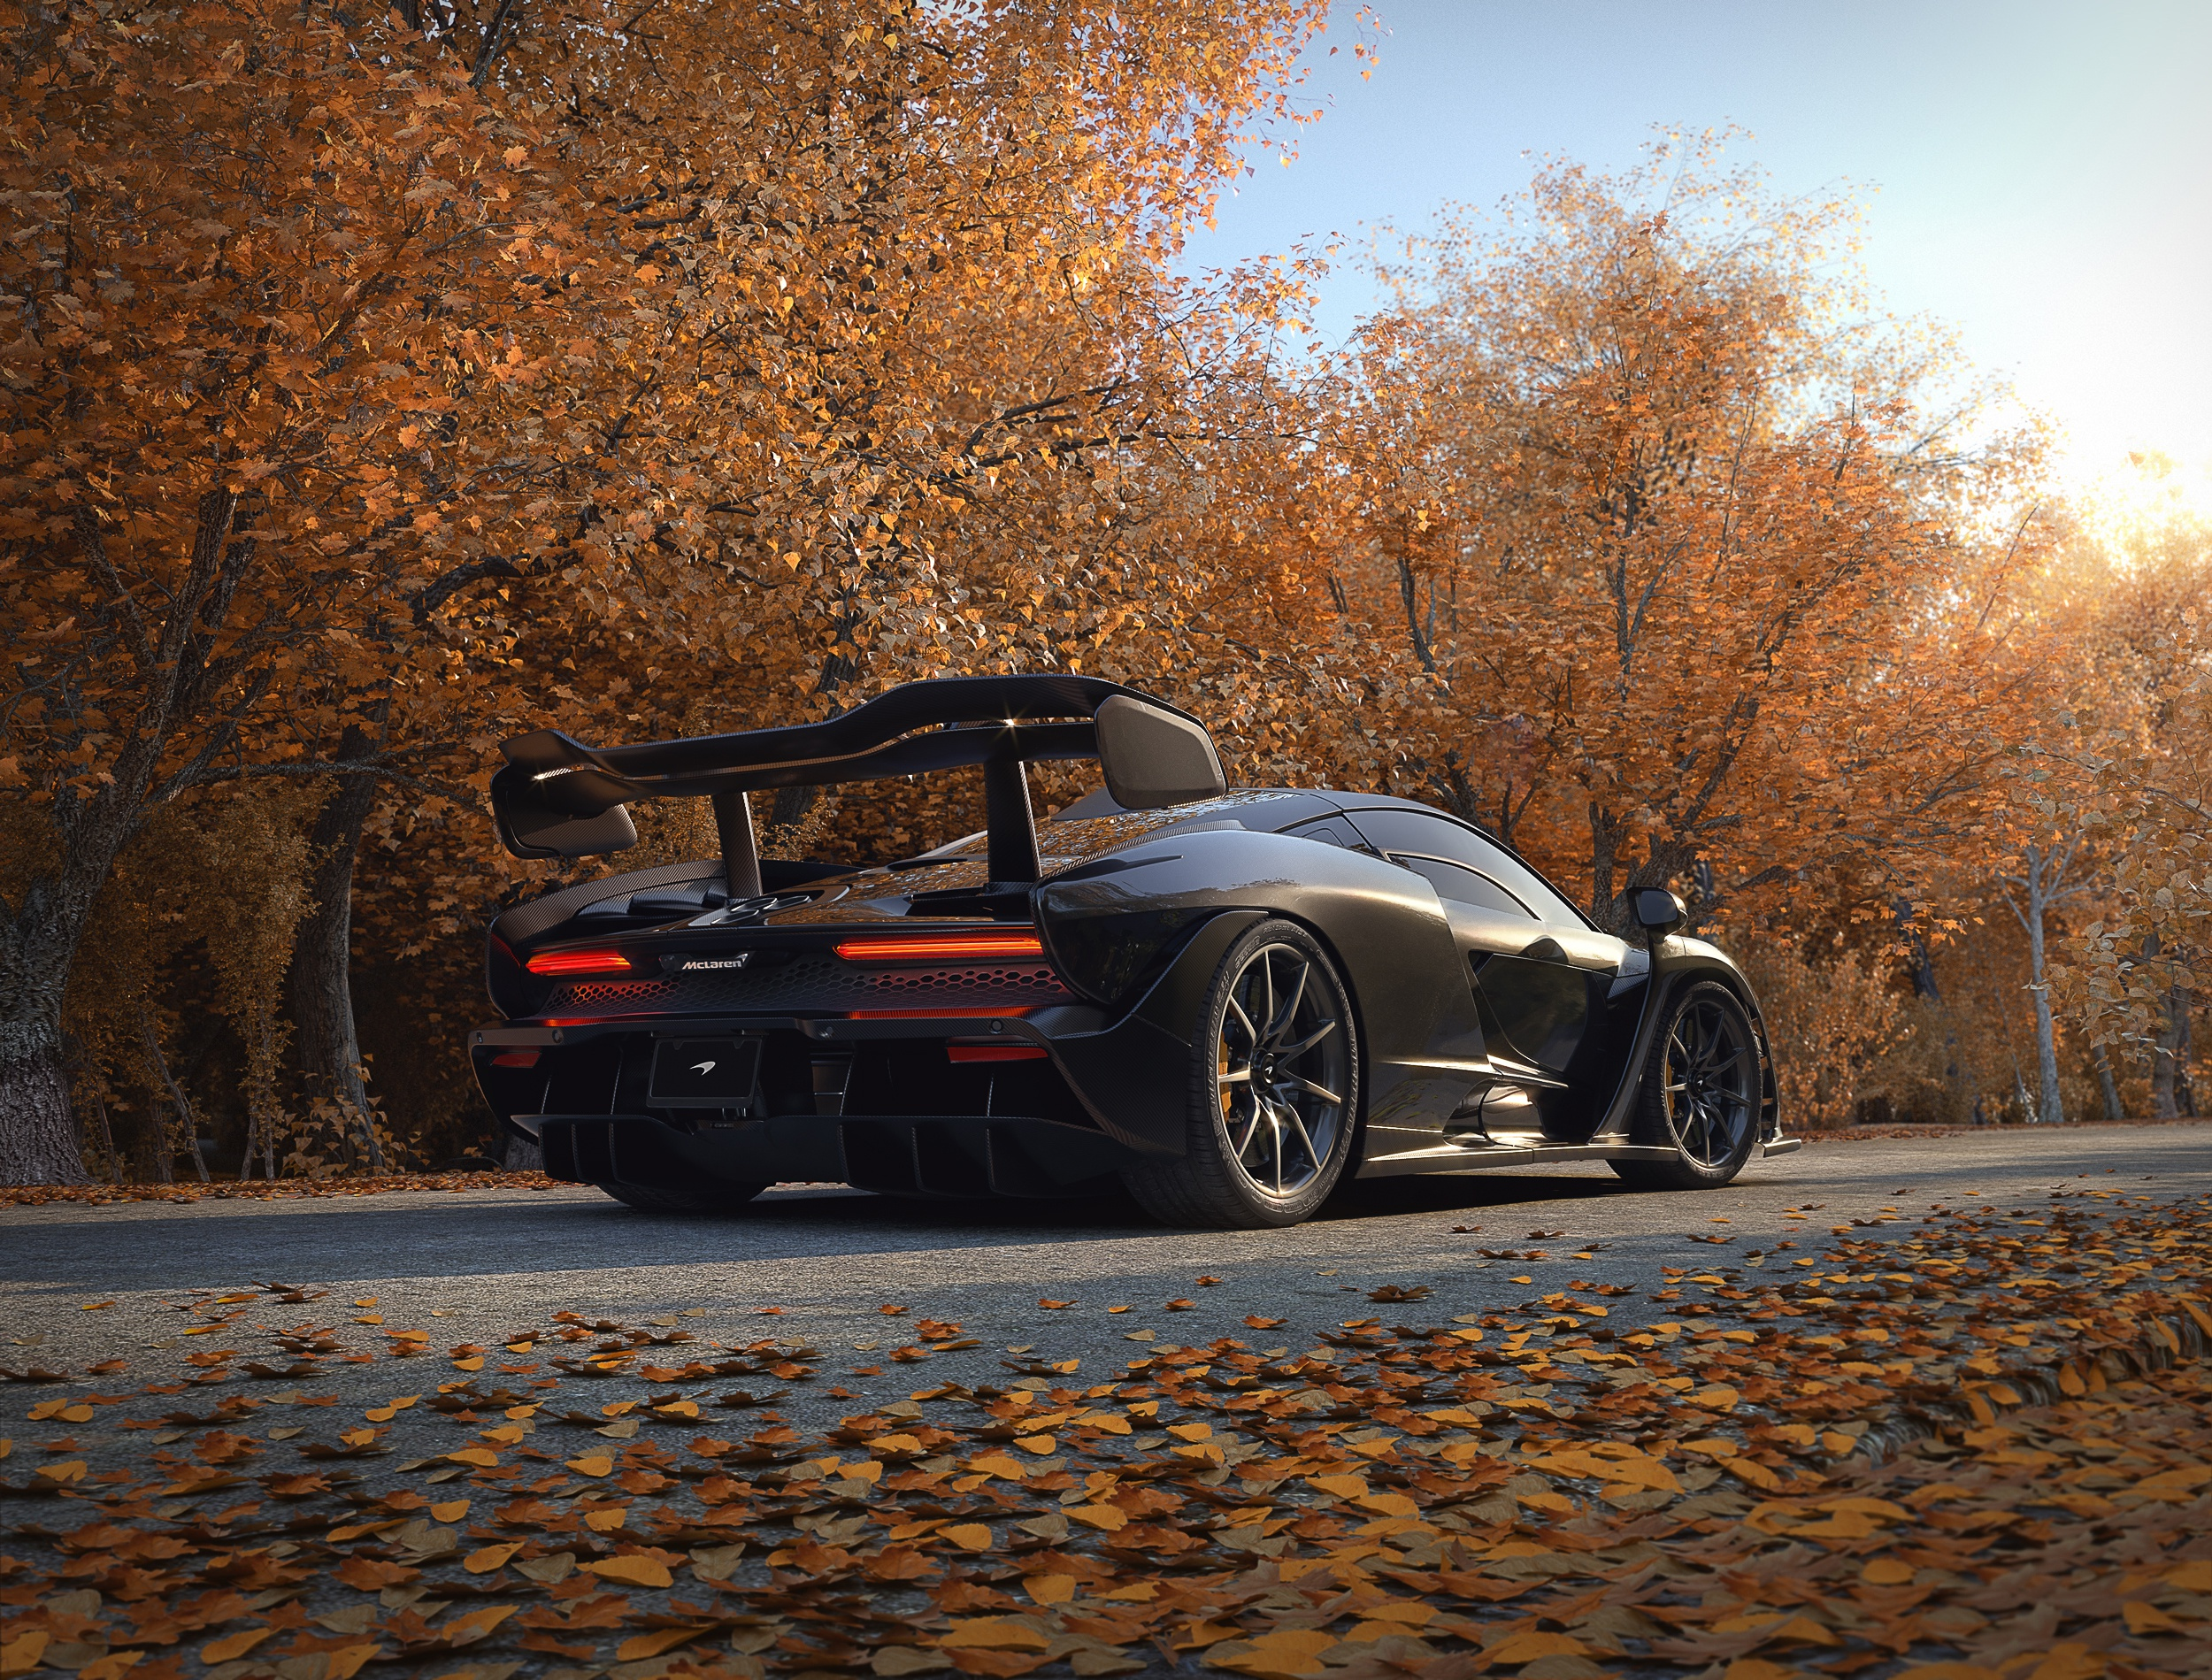
\includegraphics[width=0.7\textwidth]{assets/McLaren Senna.jpg}
    \caption{Descripción de la imagen}
    \label{fig:mi_imagen}
    \end{figure}

    % Dos imágenes lado a lado, cada una con su respectiva leyenda y etiqueta para referenciarla en el texto.
    \begin{figure}[h]
    \centering
    \begin{minipage}{0.45\textwidth}
        \centering
        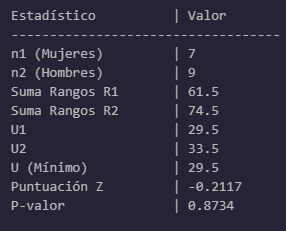
\includegraphics[width=\textwidth]{assets/1 (1).png}
        \caption{Primera imagen}
        \label{fig:imagen1}
    \end{minipage}
    \hfill
    \begin{minipage}{0.45\textwidth}
        \centering
        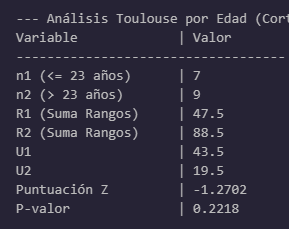
\includegraphics[width=\textwidth]{assets/1 (2).png}
        \caption{Segunda imagen}
        \label{fig:imagen2}
    \end{minipage}
    \end{figure}
    % Dos imágenes lado a lado, pero con un único caption para ambas y una etiqueta para referenciar a ambas imágenes en el texto.
    \begin{figure}[h]
    \centering
    \begin{minipage}{0.45\textwidth}
        \centering
        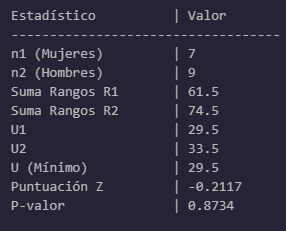
\includegraphics[width=\textwidth]{assets/1 (1).png}
    \end{minipage}
    \hfill
    \begin{minipage}{0.45\textwidth}
        \centering
        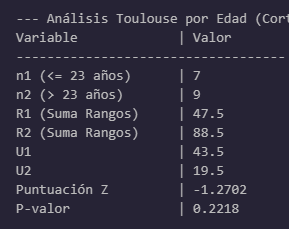
\includegraphics[width=\textwidth]{assets/1 (2).png}
    \end{minipage}
    \caption{Ambas imágenes con un único caption}
    \label{fig:ambas}
\end{figure}

\begin{multicols}{2}
    Lorem ipsum dolor sit amet, consectetur adipiscing elit. 
    Sed do eiusmod tempor incididunt ut labore et dolore magna aliqua. 
    Ut enim ad minim veniam, quis nostrud exercitation ullamco laboris 
    nisi ut aliquip ex ea commodo consequat. Duis aute irure dolor in 
    reprehenderit in voluptate velit esse cillum dolore eu fugiat nulla pariatur.
\end{multicols}

\begin{multicols}{2}
    \textbf{Primera columna}\\
    Lorem ipsum dolor sit amet, consectetur adipiscing elit. 
    Sed do eiusmod tempor incididunt ut labore et dolore magna aliqua. 
    Ut enim ad minim veniam, quis nostrud exercitation ullamco laboris 
    nisi ut aliquip ex ea commodo consequat.
    
    \columnbreak
    \textbf{Primera columna}\\
    Aquí comienza la segunda columna. Duis aute irure dolor in 
    reprehenderit in voluptate velit esse cillum dolore eu fugiat nulla pariatur.
    Excepteur sint occaecat cupidatat non proident, sunt in culpa qui officia 
    deserunt mollit anim id est laborum.
\end{multicols}
% Una imagen a la izquierda y texto a la derecha, ambos con su respectiva leyenda y etiqueta para referenciar en el texto.
\begin{figure}[h]
    \begin{center}
        \begin{minipage}{0.48\textwidth}
            \centering
            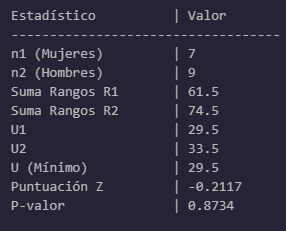
\includegraphics[width=\textwidth]{assets/1 (1).png}
            \captionsetup{justification=raggedright,singlelinecheck=false}
            \captionof{figure}{Descripción de la imagen}
            \label{fig:imagen_columna}
        \end{minipage}
        \hspace{0.5cm}
        \begin{minipage}{0.48\textwidth}
            \textbf{Título del texto}
            
            Lorem ipsum dolor sit amet, consectetur adipiscing elit. Praesent sed sem ultricies, 
            tincidunt purus eu, imperdiet enim. Duis scelerisque, quam ut placerat laoreet, leo 
            lectus placerat enim, eget condimentum magna magna sed dolor. Sed suscipit accumsan nulla. 
            Nam pharetra leo interdum nulla euismod, sed ornare ligula aliquam. Nulla ut lectus 
            fringilla purus tempor tristique nec id erat. Curabitur sed dui efficitur, placerat nisl non, 
            cursus elit. Donec ut suscipit libero, vitae finibus tortor. In vel ligula arcu. Vestibulum 
            ante ipsum primis in faucibus orci luctus et ultrices posuere cubilia curae; Morbi eros lorem, 
            efficitur a nibh eu, sodales blandit sapien. Mauris lacinia eu neque sit amet molestie. 
            In imperdiet eu tortor ut volutpat. Nullam blandit nulla sed molestie ultrices. Nullam id 
            ante magna.
        \end{minipage}
    \end{center}
    %\caption{Descripción de ambas cosas}
    %\label{fig:imagen_columna}
\end{figure}

\FloatBarrier  % Como las figuras son flotantes, esta línea asegura que todo lo anterior se imprima antes de continuar con el texto siguiente.
% \clearpage también se puede usar, pero \FloatBarrier es más específico para este caso.
Lorem ipsum dolor sit amet, consectetur adipiscing elit. Vestibulum sodales, ligula sit amet pellentesque 
elementum, urna lorem vestibulum ligula, sed consequat sem nulla quis sapien. In hac habitasse platea dictumst. 
Vestibulum sed porta quam. Orci varius natoque penatibus et magnis dis parturient montes, nascetur ridiculus mus. 
Phasellus mauris nibh, rhoncus in tortor id, eleifend luctus orci. Nam placerat, dui et faucibus efficitur, 
nulla libero volutpat magna, semper mattis arcu est ut nunc. Nunc posuere bibendum mauris ac consectetur. 
Nullam sodales vel dui a mattis. Integer at nibh consequat, dictum sapien non, faucibus purus. Vivamus id mi a 
lacus blandit tincidunt non ac orci. Aliquam non ligula felis. Nam molestie ut elit ut tempor. Pellentesque 
luctus, urna ac rhoncus volutpat, urna leo tristique turpis, et dictum ligula purus lacinia elit.


\begin{table}[h]
                \centering
                \caption{Registro de evaluación}
                \renewcommand{\arraystretch}{1.5} % 1 es el normal, 1.5 es ideal
                \begin{tabular}{|l|c|c|r|} % Las barras '|' crean las líneas verticales
                    \hline % Línea horizontal superior
                    Nombre & Evaluación & Inasistencia & Evaluación total\\ \hline \hline
                    Garrido Vázquez Fernanda          & 15                 & 25\%            &\\ \hline
                    Clase 2          & 30                 & 50\%            &\\ \hline
                    Clase 3          & 15                 & 25\%            &\\ \hline
                    Total            & 60                 & 100\%           &\\ \hline
                \end{tabular}
\end{table} \vspace{0.8cm}


\end{document}